\PassOptionsToPackage{unicode=true}{hyperref} % options for packages loaded elsewhere
\PassOptionsToPackage{hyphens}{url}
%
\documentclass[]{article}
\usepackage{lmodern}
\usepackage{amssymb,amsmath}
\usepackage{ifxetex,ifluatex}
\usepackage{fixltx2e} % provides \textsubscript
\ifnum 0\ifxetex 1\fi\ifluatex 1\fi=0 % if pdftex
  \usepackage[T1]{fontenc}
  \usepackage[utf8]{inputenc}
  \usepackage{textcomp} % provides euro and other symbols
\else % if luatex or xelatex
  \usepackage{unicode-math}
  \defaultfontfeatures{Ligatures=TeX,Scale=MatchLowercase}
\fi
% use upquote if available, for straight quotes in verbatim environments
\IfFileExists{upquote.sty}{\usepackage{upquote}}{}
% use microtype if available
\IfFileExists{microtype.sty}{%
\usepackage[]{microtype}
\UseMicrotypeSet[protrusion]{basicmath} % disable protrusion for tt fonts
}{}
\IfFileExists{parskip.sty}{%
\usepackage{parskip}
}{% else
\setlength{\parindent}{0pt}
\setlength{\parskip}{6pt plus 2pt minus 1pt}
}
\usepackage{hyperref}
\hypersetup{
            pdftitle={STAT 385 Learning Progress},
            pdfauthor={Bradley Simon},
            pdfborder={0 0 0},
            breaklinks=true}
\urlstyle{same}  % don't use monospace font for urls
\usepackage[margin=1in]{geometry}
\usepackage{color}
\usepackage{fancyvrb}
\newcommand{\VerbBar}{|}
\newcommand{\VERB}{\Verb[commandchars=\\\{\}]}
\DefineVerbatimEnvironment{Highlighting}{Verbatim}{commandchars=\\\{\}}
% Add ',fontsize=\small' for more characters per line
\usepackage{framed}
\definecolor{shadecolor}{RGB}{248,248,248}
\newenvironment{Shaded}{\begin{snugshade}}{\end{snugshade}}
\newcommand{\AlertTok}[1]{\textcolor[rgb]{0.94,0.16,0.16}{#1}}
\newcommand{\AnnotationTok}[1]{\textcolor[rgb]{0.56,0.35,0.01}{\textbf{\textit{#1}}}}
\newcommand{\AttributeTok}[1]{\textcolor[rgb]{0.77,0.63,0.00}{#1}}
\newcommand{\BaseNTok}[1]{\textcolor[rgb]{0.00,0.00,0.81}{#1}}
\newcommand{\BuiltInTok}[1]{#1}
\newcommand{\CharTok}[1]{\textcolor[rgb]{0.31,0.60,0.02}{#1}}
\newcommand{\CommentTok}[1]{\textcolor[rgb]{0.56,0.35,0.01}{\textit{#1}}}
\newcommand{\CommentVarTok}[1]{\textcolor[rgb]{0.56,0.35,0.01}{\textbf{\textit{#1}}}}
\newcommand{\ConstantTok}[1]{\textcolor[rgb]{0.00,0.00,0.00}{#1}}
\newcommand{\ControlFlowTok}[1]{\textcolor[rgb]{0.13,0.29,0.53}{\textbf{#1}}}
\newcommand{\DataTypeTok}[1]{\textcolor[rgb]{0.13,0.29,0.53}{#1}}
\newcommand{\DecValTok}[1]{\textcolor[rgb]{0.00,0.00,0.81}{#1}}
\newcommand{\DocumentationTok}[1]{\textcolor[rgb]{0.56,0.35,0.01}{\textbf{\textit{#1}}}}
\newcommand{\ErrorTok}[1]{\textcolor[rgb]{0.64,0.00,0.00}{\textbf{#1}}}
\newcommand{\ExtensionTok}[1]{#1}
\newcommand{\FloatTok}[1]{\textcolor[rgb]{0.00,0.00,0.81}{#1}}
\newcommand{\FunctionTok}[1]{\textcolor[rgb]{0.00,0.00,0.00}{#1}}
\newcommand{\ImportTok}[1]{#1}
\newcommand{\InformationTok}[1]{\textcolor[rgb]{0.56,0.35,0.01}{\textbf{\textit{#1}}}}
\newcommand{\KeywordTok}[1]{\textcolor[rgb]{0.13,0.29,0.53}{\textbf{#1}}}
\newcommand{\NormalTok}[1]{#1}
\newcommand{\OperatorTok}[1]{\textcolor[rgb]{0.81,0.36,0.00}{\textbf{#1}}}
\newcommand{\OtherTok}[1]{\textcolor[rgb]{0.56,0.35,0.01}{#1}}
\newcommand{\PreprocessorTok}[1]{\textcolor[rgb]{0.56,0.35,0.01}{\textit{#1}}}
\newcommand{\RegionMarkerTok}[1]{#1}
\newcommand{\SpecialCharTok}[1]{\textcolor[rgb]{0.00,0.00,0.00}{#1}}
\newcommand{\SpecialStringTok}[1]{\textcolor[rgb]{0.31,0.60,0.02}{#1}}
\newcommand{\StringTok}[1]{\textcolor[rgb]{0.31,0.60,0.02}{#1}}
\newcommand{\VariableTok}[1]{\textcolor[rgb]{0.00,0.00,0.00}{#1}}
\newcommand{\VerbatimStringTok}[1]{\textcolor[rgb]{0.31,0.60,0.02}{#1}}
\newcommand{\WarningTok}[1]{\textcolor[rgb]{0.56,0.35,0.01}{\textbf{\textit{#1}}}}
\usepackage{graphicx,grffile}
\makeatletter
\def\maxwidth{\ifdim\Gin@nat@width>\linewidth\linewidth\else\Gin@nat@width\fi}
\def\maxheight{\ifdim\Gin@nat@height>\textheight\textheight\else\Gin@nat@height\fi}
\makeatother
% Scale images if necessary, so that they will not overflow the page
% margins by default, and it is still possible to overwrite the defaults
% using explicit options in \includegraphics[width, height, ...]{}
\setkeys{Gin}{width=\maxwidth,height=\maxheight,keepaspectratio}
\setlength{\emergencystretch}{3em}  % prevent overfull lines
\providecommand{\tightlist}{%
  \setlength{\itemsep}{0pt}\setlength{\parskip}{0pt}}
\setcounter{secnumdepth}{0}
% Redefines (sub)paragraphs to behave more like sections
\ifx\paragraph\undefined\else
\let\oldparagraph\paragraph
\renewcommand{\paragraph}[1]{\oldparagraph{#1}\mbox{}}
\fi
\ifx\subparagraph\undefined\else
\let\oldsubparagraph\subparagraph
\renewcommand{\subparagraph}[1]{\oldsubparagraph{#1}\mbox{}}
\fi

% set default figure placement to htbp
\makeatletter
\def\fps@figure{htbp}
\makeatother


\title{STAT 385 Learning Progress}
\author{Bradley Simon}
\date{2020-03-04}

\begin{document}
\maketitle

The first topics I learned in R were basic mathematical operations,
creating functions, data types, data structures, and data frames. One of
the first functions I created was a French Roulette wheel that returns
whether the user's input bet wins or not. The code for this function is
shown below.

\begin{Shaded}
\begin{Highlighting}[]
\NormalTok{wheel <-}\StringTok{ }\KeywordTok{read.csv}\NormalTok{(}\StringTok{"https://nkha149.github.io/stat385-sp2020/files/data/roulette.csv"}\NormalTok{)}
\NormalTok{roulette <-}\StringTok{ }\ControlFlowTok{function}\NormalTok{(}\DataTypeTok{bet =} \DecValTok{14}\NormalTok{) \{}
\NormalTok{  win_num <-}\StringTok{ }\KeywordTok{sample}\NormalTok{(}\DataTypeTok{x =} \DecValTok{1}\OperatorTok{:}\DecValTok{37}\NormalTok{, }\DataTypeTok{size =} \DecValTok{1}\NormalTok{)}
\NormalTok{  wheel[win_num, }\DecValTok{1}\NormalTok{] }\OperatorTok{==}\StringTok{ }\NormalTok{bet}
\NormalTok{\}}
\KeywordTok{set.seed}\NormalTok{(}\DecValTok{385}\NormalTok{)}
\KeywordTok{roulette}\NormalTok{(}\DataTypeTok{bet =} \DecValTok{10}\NormalTok{)}
\end{Highlighting}
\end{Shaded}

\begin{verbatim}
## [1] FALSE
\end{verbatim}

I have also learned how to modify vlaues in lists, vectors, matrices,
and data frames, as well as how to graph data sets. The code for a
scatterplot that is categroized by color is shown below.

\begin{Shaded}
\begin{Highlighting}[]
\KeywordTok{plot}\NormalTok{(}\DataTypeTok{formula =}\NormalTok{ Sepal.Width }\OperatorTok{~}\StringTok{ }\NormalTok{Sepal.Length, }\DataTypeTok{data =}\NormalTok{ iris,}
     \DataTypeTok{col =} \KeywordTok{c}\NormalTok{(}\StringTok{"green"}\NormalTok{, }\StringTok{"red"}\NormalTok{, }\StringTok{"blue"}\NormalTok{)[iris}\OperatorTok{$}\NormalTok{Species],}
     \DataTypeTok{main =} \StringTok{"Iris Sepal Length vs. Sepal Width by Species"}\NormalTok{,}
     \DataTypeTok{xlab =} \StringTok{"Sepal Length"}\NormalTok{, }\DataTypeTok{ylab =} \StringTok{"Sepal Width"}\NormalTok{, }\DataTypeTok{pch =} \DecValTok{16}\NormalTok{)}
\KeywordTok{grid}\NormalTok{()}
\end{Highlighting}
\end{Shaded}

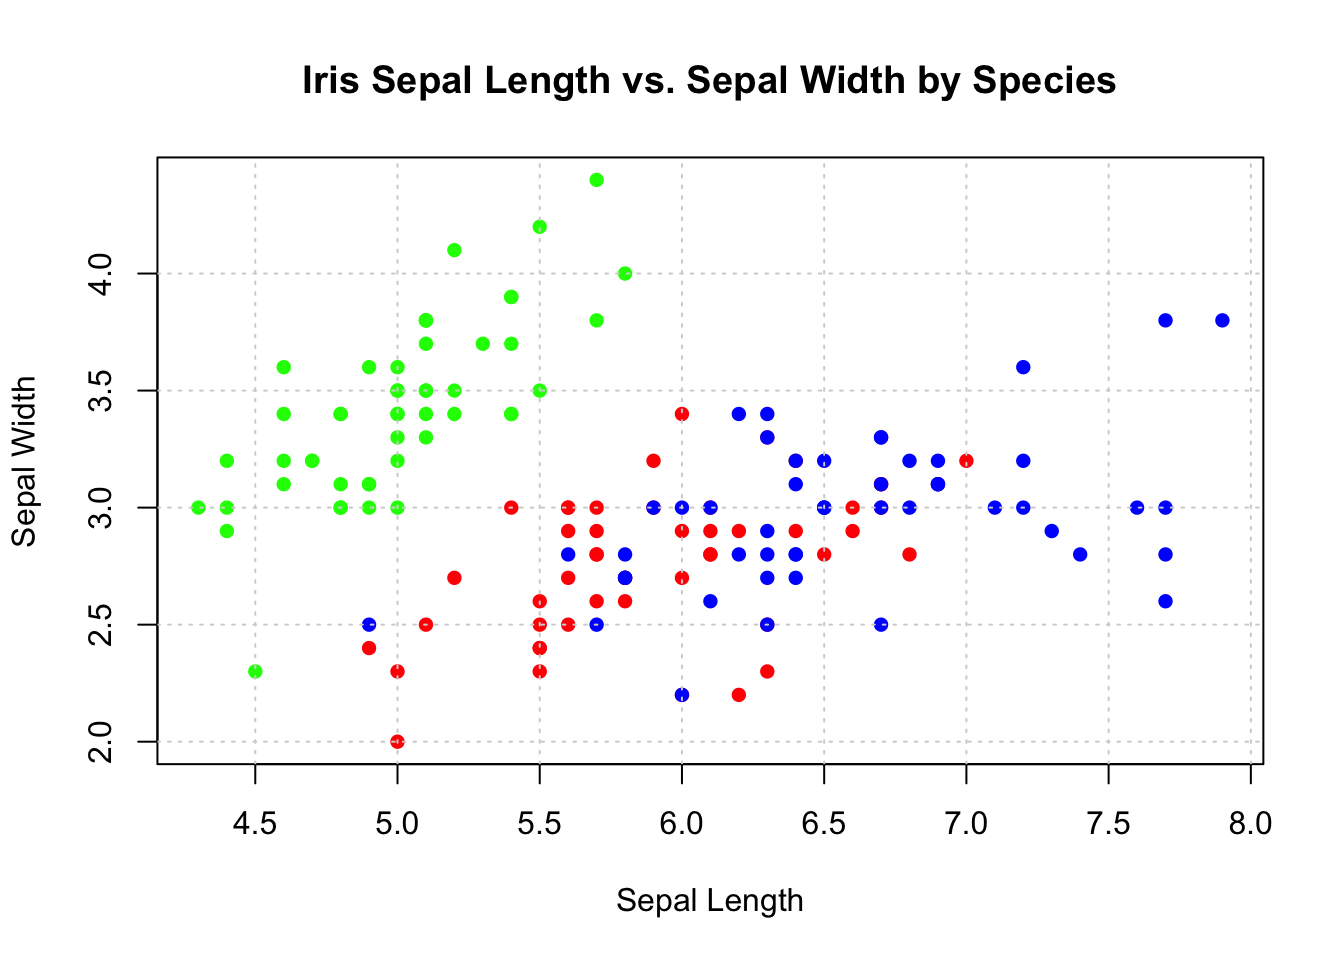
\includegraphics{2020-03-04-stat-385-learning-progress_files/figure-latex/unnamed-chunk-2-1.pdf}

Lastly, I have learned how to utilize parellel computing by vectorizing
functions. I took the loop function shown below and vectorized it so
that the speed was increased significantly.

\begin{Shaded}
\begin{Highlighting}[]
\NormalTok{roulette_loop <-}\StringTok{ }\ControlFlowTok{function}\NormalTok{(many_bets) \{}
\NormalTok{  win_lose_random <-}\StringTok{ }\KeywordTok{sample}\NormalTok{(}\DataTypeTok{x =} \KeywordTok{c}\NormalTok{(}\OtherTok{TRUE}\NormalTok{, }\OtherTok{FALSE}\NormalTok{), }\DataTypeTok{size =} \KeywordTok{length}\NormalTok{(many_bets),}
                            \DataTypeTok{replace =} \OtherTok{TRUE}\NormalTok{)}
\NormalTok{  total_prize <-}\StringTok{ }\KeywordTok{c}\NormalTok{()}
  \ControlFlowTok{for}\NormalTok{ (i }\ControlFlowTok{in} \DecValTok{1}\OperatorTok{:}\KeywordTok{length}\NormalTok{(many_bets)) \{}
\NormalTok{    bet <-}\StringTok{ }\NormalTok{many_bets[i]}
\NormalTok{    prize <-}\StringTok{ }\DecValTok{0}
    \ControlFlowTok{if}\NormalTok{ (win_lose_random[i]) \{}
      \ControlFlowTok{if}\NormalTok{ (bet }\OperatorTok{==}\StringTok{ 'low'}\NormalTok{) \{}
\NormalTok{        prize <-}\StringTok{ }\DecValTok{10}
\NormalTok{      \} }\ControlFlowTok{else} \ControlFlowTok{if}\NormalTok{ (bet }\OperatorTok{==}\StringTok{ 'high'}\NormalTok{)\{}
\NormalTok{        prize <-}\StringTok{ }\DecValTok{10}
\NormalTok{      \} }\ControlFlowTok{else} \ControlFlowTok{if}\NormalTok{ (bet }\OperatorTok{==}\StringTok{ 'red'}\NormalTok{) \{}
\NormalTok{        prize <-}\StringTok{ }\DecValTok{20}
\NormalTok{      \} }\ControlFlowTok{else} \ControlFlowTok{if}\NormalTok{ (bet }\OperatorTok{==}\StringTok{ "black"}\NormalTok{) \{}
\NormalTok{        prize <-}\StringTok{ }\DecValTok{20}
\NormalTok{      \} }\ControlFlowTok{else} \ControlFlowTok{if}\NormalTok{ (bet }\OperatorTok{==}\StringTok{ "odd"}\NormalTok{) \{}
\NormalTok{        prize <-}\StringTok{ }\DecValTok{15}
\NormalTok{      \} }\ControlFlowTok{else} \ControlFlowTok{if}\NormalTok{ (bet }\OperatorTok{==}\StringTok{ "even"}\NormalTok{) \{}
\NormalTok{        prize <-}\StringTok{ }\DecValTok{15}
\NormalTok{      \} }\ControlFlowTok{else} \ControlFlowTok{if}\NormalTok{ (bet }\OperatorTok{==}\StringTok{ "first"}\NormalTok{) \{}
\NormalTok{        prize <-}\StringTok{ }\DecValTok{50}
\NormalTok{      \} }\ControlFlowTok{else} \ControlFlowTok{if}\NormalTok{ (bet }\OperatorTok{==}\StringTok{ "second"}\NormalTok{) \{}
\NormalTok{        prize <-}\StringTok{ }\DecValTok{50}
\NormalTok{      \} }\ControlFlowTok{else} \ControlFlowTok{if}\NormalTok{ (bet }\OperatorTok{==}\StringTok{ "third"}\NormalTok{) \{}
\NormalTok{        prize <-}\StringTok{ }\DecValTok{50}
\NormalTok{      \}}
\NormalTok{    \}}
\NormalTok{  total_prize <-}\StringTok{ }\KeywordTok{c}\NormalTok{(total_prize, prize)}
\NormalTok{  \}}
  
\NormalTok{  total_prize}
\NormalTok{\}}
\KeywordTok{set.seed}\NormalTok{(}\DecValTok{385}\NormalTok{)}
\NormalTok{long_vec <-}\StringTok{ }\KeywordTok{rep}\NormalTok{(}\KeywordTok{c}\NormalTok{(}\StringTok{"red"}\NormalTok{, }\StringTok{"black"}\NormalTok{, }\StringTok{"low"}\NormalTok{, }\StringTok{"high"}\NormalTok{, }\StringTok{"second"}\NormalTok{, }\StringTok{"first"}\NormalTok{, }\StringTok{"third"}\NormalTok{,}
                  \StringTok{"odd"}\NormalTok{, }\StringTok{"even"}\NormalTok{), }\DecValTok{10000}\NormalTok{)}
\KeywordTok{system.time}\NormalTok{(}\KeywordTok{roulette_loop}\NormalTok{(}\DataTypeTok{many_bets =}\NormalTok{ long_vec))}
\end{Highlighting}
\end{Shaded}

\begin{verbatim}
##    user  system elapsed 
##  18.769  10.766  29.580
\end{verbatim}

\begin{Shaded}
\begin{Highlighting}[]
\NormalTok{roulette_vec <-}\StringTok{ }\ControlFlowTok{function}\NormalTok{(many_bets)\{}
\NormalTok{  win_lose_random <-}\StringTok{ }\KeywordTok{sample}\NormalTok{(}\DataTypeTok{x =} \KeywordTok{c}\NormalTok{(}\OtherTok{TRUE}\NormalTok{, }\OtherTok{FALSE}\NormalTok{), }\DataTypeTok{size =} \KeywordTok{length}\NormalTok{(many_bets),}
                            \DataTypeTok{replace =} \OtherTok{TRUE}\NormalTok{)}
\NormalTok{  look_up_table <-}\StringTok{ }\KeywordTok{c}\NormalTok{(}\StringTok{"low"}\NormalTok{ =}\StringTok{ }\DecValTok{10}\NormalTok{,}\StringTok{"high"}\NormalTok{ =}\StringTok{ }\DecValTok{10}\NormalTok{, }\StringTok{"red"}\NormalTok{ =}\StringTok{ }\DecValTok{20}\NormalTok{, }\StringTok{"black"}\NormalTok{ =}\StringTok{ }\DecValTok{20}\NormalTok{, }\StringTok{"odd"}\NormalTok{ =}\StringTok{   }\DecValTok{15}\NormalTok{,}\StringTok{"even"}\NormalTok{ =}\StringTok{ }\DecValTok{15}\NormalTok{,}
                     \StringTok{"first"}\NormalTok{ =}\StringTok{ }\DecValTok{50}\NormalTok{, }\StringTok{"second"}\NormalTok{ =}\StringTok{ }\DecValTok{50}\NormalTok{, }\StringTok{"third"}\NormalTok{ =}\StringTok{ }\DecValTok{50}\NormalTok{)}
\NormalTok{  prize <-}\StringTok{ }\NormalTok{look_up_table[many_bets]}
  \KeywordTok{unname}\NormalTok{(win_lose_random }\OperatorTok{*}\StringTok{ }\NormalTok{prize)}
\NormalTok{\}}


\KeywordTok{set.seed}\NormalTok{(}\DecValTok{385}\NormalTok{)}
\NormalTok{long_vec <-}\StringTok{ }\KeywordTok{rep}\NormalTok{(}\KeywordTok{c}\NormalTok{(}\StringTok{"red"}\NormalTok{, }\StringTok{"black"}\NormalTok{, }\StringTok{"low"}\NormalTok{, }\StringTok{"high"}\NormalTok{, }\StringTok{"second"}\NormalTok{, }\StringTok{"first"}\NormalTok{, }\StringTok{"third"}\NormalTok{,}
                  \StringTok{"odd"}\NormalTok{, }\StringTok{"even"}\NormalTok{), }\DecValTok{10000}\NormalTok{)}
\KeywordTok{system.time}\NormalTok{(}\KeywordTok{roulette_vec}\NormalTok{(}\DataTypeTok{many_bets =}\NormalTok{ long_vec))}
\end{Highlighting}
\end{Shaded}

\begin{verbatim}
##    user  system elapsed 
##   0.007   0.000   0.008
\end{verbatim}

\end{document}
